%-----------------------------------------------------------------
%	SEMI-CLASSICAL LIGHT DESCRIPTION
%	!TEX root = ./../main.tex
%----------------------------------------------------------------
\section{Semi-classical light description}
\subsection{Maxwell's equations}
Maxwell's equations are a set of partial differential equations that, together with the Lorentz force Law, form the foundation of classical electrodynamics, classical optics, and electric circuits:
\begin{align}
	\div{D} &= \rho_{free} \tag{Gauss's law} \\
	\div{B} &= 0 \tag{Gauss's law for magnetism} \\
	\curl{E} &= - \pdv{\va{B}}{t} \tag{Faraday's law} \\
	\curl{B} &= \va{J}_{free} + \pdv{\va{D}}{t} \tag{Ampère's law}
\end{align}

Apart from Maxwell's equations themselves, it's important to remember the following relationships for the electric and magnetic fields:
\begin{align*}
	\va{D} = \varepsilon \va{E} + \va{P} \qc \va{B} = \mu_{0} \va{H} + \va{M}
\end{align*}

\subsubsection*{Wave equation}
The general form of the wave wave equation is:
\begin{align*}
	- \laplacian{\va{E}} + \mu_{0} \dv{\va{J}_{free}}{t} + \frac{1}{c^{2}} \dv[2]{\va{E}}{t} = - \mu_{0} \dv[2]{\va{P}}{t}
\end{align*}
However, considering the properties of optical materials ($\rho_{free} = 0$, $\va{M} = \va{0}$, $\mu \approx \mu_{0}$, and $\va{J}_{free} = \va{0}$), we can simplify it and rewrite it as
\begin{align}
	\laplacian{\va{E}} - \frac{1}{c^{2}} \dv[2]{\va{E}}{t} = \mu_{0} \dv[2]{\va{P}}{t}
\end{align}

%-----------------------------------------------------------------
\subsection[Slowly varying envelope approximation]{Slowly varying envelope approximation (SVEA)}
The electric field can be written as
\begin{align}\label{eq:Ezt-epsilon}
	\va{E}(z,t) = \vu{\varepsilon}\, E_{0}(z,t) e^{i(kz - \omega t - \phi(z,t))} = \vu{\varepsilon}\, \mc{E}_{0}(z,t) e^{-i \omega t}
\end{align}
where $\vu{\varepsilon}$ is the unit polarisation vector, and $\mc{E}_{0}$ is the amplitude of the electric field; $E_{0}(z,t)$ and $\phi(z,t)$ are slowly varying functions. Of course, due to a possible phase lag of the medium, the polarization phase may have a phase different from that of the field. In this case, slowly varying means
\begin{align*}
	\left.
	\begin{aligned}
		\abs{\dv{E_{0}}{z}} &\ll \frac{E_{0}}{\lambda} \sim E_{0} k \\
		\abs{\dv{E_{0}}{t}} &\ll \frac{E_{0}}{T} \sim E_{0} \omega
	\end{aligned}
	\right\}
	\qand
	\left\{
	\begin{aligned}
		\abs{\dv{\phi}{z}} &\ll \frac{2 \pi}{\lambda} \sim k \\
		\abs{\dv{\phi}{t}} &\ll \frac{2 \pi}{T} \sim \omega
	\end{aligned}
	\right.
\end{align*}
The slowly varying envelope approximation, thus, is the assumption that the envelope of a forward-travelling wave pulse varies slowly in time and space compared to a period or wavelength. As a result of the slow variation of these functions, when taking derivatives, the highest-order derivatives may be neglected.

Let's consider the wave function in the vacuum, $\dsp \laplacian{\va{E}} - \frac{1}{c^{2}} \dv[2]{\va{E}}{t} = 0$. Since $\va{E} = \va{E}(z,t)$, this becomes
\begin{align}
	\dv[2]{\va{E}}{z} - \frac{1}{c^{2}} \dv[2]{\va{E}}{t} = 0
\end{align}
Following the expression for $\va{E}(z,t)$ in the equation \eqref{eq:Ezt-epsilon}, and deriving the equation above, we get
\begin{align*}
\begin{aligned}
	2i E_{0} (k - \phi') &+ E_{0}'' - i E_{0} \phi'' - E_{0} (k - \phi')^{2} \\
	&= \frac{1}{c^{2}} \qty[ -2i \dot{E}_{0} (\omega + \dot{\phi}) + \ddot{E}_{0} - i E_{0} \ddot{\phi} - E_{0} (\omega + \dot{\phi})^{2}]
\end{aligned}
\end{align*}

Let's apply the slowly varying envelope approximation. On one hand, for the imaginary part of the expression above, we get
\begin{flalign*}
	2 E_{0} \tikzmark{a}k - 2 \tikzmark{b}E_{0} \tikzmark{c}\phi' - E_{0}\tikzmark{d} \phi'' &= \dfrac{1}{c^{2}} \qty[ - 2 \dot{E}_{0} \tikzmark{e}\omega - 2 \tikzmark{f}\dot{E}_{0} \tikzmark{g}\dot{\phi} - i E_{0} \tikzmark{h}\ddot{\phi}] \Rightarrow E_{0}' = - \frac{1}{c} \dot{E}_{0} & \\
	\tikz[overlay,remember picture,label distance=10pt]{\path[draw, <-, square arrow] (a.south) to (b.south); \node[label=below:\footnotesize{SVEA}] at ($ (a) !.5! (b) $) {};}
	\tikz[overlay,remember picture,label distance=10pt]{\path[draw, <-, square arrow] (c.south) to (d.south); \node[label=below:\footnotesize{$\order*{\phi''}$}] at ($ (c) !.5! (d) $) {};}
	\tikz[overlay,remember picture,label distance=10pt]{\path[draw, <-, square arrow] (e.south) to (f.south); \node[label=below:\footnotesize{SVEA}] at ($ (e) !.5! (f) $) {};}
	\tikz[overlay,remember picture,label distance=10pt]{\path[draw, <-, square arrow] (g.south) to (h.south); \node[label=below:\footnotesize{$\order*{\ddot{\phi}}$}] at ($ (g) !.5! (h) $) {};}
\end{flalign*}
On the other hand, for the real part, we get
\begin{flalign*}
	E_{0}'' &- E_{0}(k - \phi')^{2} = \dfrac{1}{c^{2}} \qty[\ddot{E}_{0} - E_{0}(\omega + \dot{\phi})^{2}] \Rightarrow - E_{0} \tikzmark{a}k^{2} + 2 E_{0} k \phi' = \dfrac{1}{c^{2}} \qty[ - E_{0} \tikzmark{b}\omega^{2} - 2 E_{0} \omega \dot{\phi}] & \\
	&\Rightarrow \phi' = - \frac{1}{c} \dot{\phi}
	\tikz[overlay,remember picture,label distance=10pt]{\path[draw, <->, square arrow] (a.south) to (b.south); \node[label=below:\footnotesize{$\equiv$}] at ($ (a) !.5! (b) $) {};}
\end{flalign*}
So, simplifying, and applying the SVEA carefully, we get separate equations for the amplitude and the phase:
\begin{align}
	E_{0}' + \frac{1}{c} \dot{E}_{0} \equiv 0 \qc \phi' + \frac{1}{c} \dot{\phi} \equiv 0
\end{align}

In the presence of a medium, we have to also consider the polarisation. The polarisation can be expressed as $\va{P}(z,t) = \vu{\varepsilon}\, \mc{P}(z,t) e^{i [kz - \omega t - \phi(z,t)]}$, where $\mc{P} \in \mbb{C}$ is the (slowly varying) polarisation amplitude. Having that in mind, and repeating the same process, we get
\begin{align}
	E_{0}' + \frac{1}{c} \dot{E}_{0} = - \frac{k}{2 \varepsilon_{0}} \Im{\mc{P}} \qc E_{0} \qty[\phi' + \frac{1}{c} \dot{\phi}] = - \frac{k}{2 \varepsilon_{0}} \Re{\mc{P}}
\end{align}

\subsubsection*{Steady situation}
In the steady situation, we know that $\dot{E}_{0} = 0$ and $\dot{\phi} = 0$. Also, considering that the polarisation amplitude can be written as $\mc{P}(z) = \varepsilon_{0} \chi E_{0}(z)$, we get
\begin{align}
	\pdv{E_{0}}{z} = - \frac{k}{2} \chi'' E_{0} \qc \pdv{\phi}{z} = - \frac{k}{2} \chi'
\end{align}

\begin{defi}[Absorption coefficient]
	The optical absorption coefficient, $\alpha$ is the most important optical constant
for photo-detectors. Its value is determined by
	\begin{align*}
		\alpha \equiv \frac{i k \chi}{2}
	\end{align*}
\end{defi}

Rewriting the equation for the spatial variation of the electric field in terms of the absorption coefficient we have $E_{0}(z) = E_{0}(0) e^{- \Re{\alpha} z}$. Therefore, we can easily get the Beer's Law:
\begin{align}
	I(z) = I(0) e^{- 2 \Re{\alpha} z}
\end{align}

Since we are in the SVEA regime, we can do a series expansion for the phase: $\phi(z) = \phi(0) + (\dv*{\phi}{z}) z$, therefore, we can rewrite the general phase $\varphi = kz - \omega t - \phi(z)$ as
\begin{flalign*}
	\varphi &= kz - \omega t - \phi (0) + k \frac{\chi'}{2} z = \omega \qty[ \qty(\frac{\chi'}{2}) \frac{z}{c} - t] - \phi(0) \Rightarrow \dd{\varphi} = 0 = \omega \qty[ \qty(\frac{\chi'}{2}) \frac{\dd{z}}{c} - \dd{t}] &
\end{flalign*}

\begin{defi}[Phase velocity]
	The phase velocity of a wave is the rate at which the phase of the wave propagates in space.
	\begin{align}
		v_{ph} \equiv \dv{z}{t} = \frac{c}{1 + \dfrac{\chi'}{2}} = \frac{c}{n (\omega)}
	\end{align}
\end{defi}

%-----------------------------------------------------------------
\subsection{Group velocity}
\begin{defi}[Wave packet]
	A wave packet is a short envelope of localized wave action that travels as a unit. A wave packet can be analysed into, or can be synthesized from, an infinite set of component sinusoidal waves of different wave numbers, with phases and amplitudes such that they interfere constructively only over a small region of space, and destructively elsewhere. For the electric field, it has the following form:
	\begin{align}
		E(z,t) = \int_{\Delta \omega} E_{\omega} e^{i (kz - \omega t)} \dd{\omega} = \underbrace{\qty[\int_{\Delta \omega} E_{\omega} e^{i [(k - k_{0})z - (\omega - \omega_{0})t]} \dd{\omega}]}_{\text{envelope of the amplitude}} \underbrace{e^{i (k_{0}z - \omega_{0} t)}}_{\text{fast oscillation}}
	\end{align}
	where $\Delta k = k - k_{0}$ and $\Delta \omega = \omega - \omega_{0}$.
\end{defi}

\begin{defi}[Group velocity]
	The group velocity of a wave is the velocity with which the overall shape of the waves' amplitudes (known as the modulation or envelope of the wave) propagates through space.
	\begin{align}
		v_{g} = \eval{\frac{\Delta z}{\Delta t}}_{maxima}
	\end{align}
\end{defi}
From the expression for the phase velocity we can see that the wave number can be written as $k = [\omega n(\omega)]/c$. Since the group velocity is defined between two maxima:
\begin{flalign*}
	\pdv{\phi}{\omega} &\equiv 0 = \Delta z \pdv{k}{\omega} - \Delta t \pdv{\omega}{\omega} \Rightarrow v_{g} = \frac{1}{\pdv*{k}{\omega}} \qc \pdv{k}{\omega} = \frac{n}{c} + \pdv{n}{\omega} \frac{\omega}{c} &
\end{flalign*}

Therefore, the group velocity can be written as
\begin{align}
		v_{g} = \frac{c}{\dsp n + \omega \pdv{n}{\omega}}
\end{align}

\subsubsection*{Slow and superluminal light}
Slow and superluminal group velocities can be observed in any material that has large normal ($\pdv*{n}{\omega} > 0$) or anomalous ($\pdv*{n}{\omega} < 0$) dispersion (figure \ref{fig:lorentz-group-vel}):
\begin{itemize}
	\item Superluminal light: $\dsp \pdv{n}{\omega} < 0$.
	\item Slow light: $\dsp \pdv{n}{\omega} > 0$.
\end{itemize}
\begin{figure}[H]
	\centering
	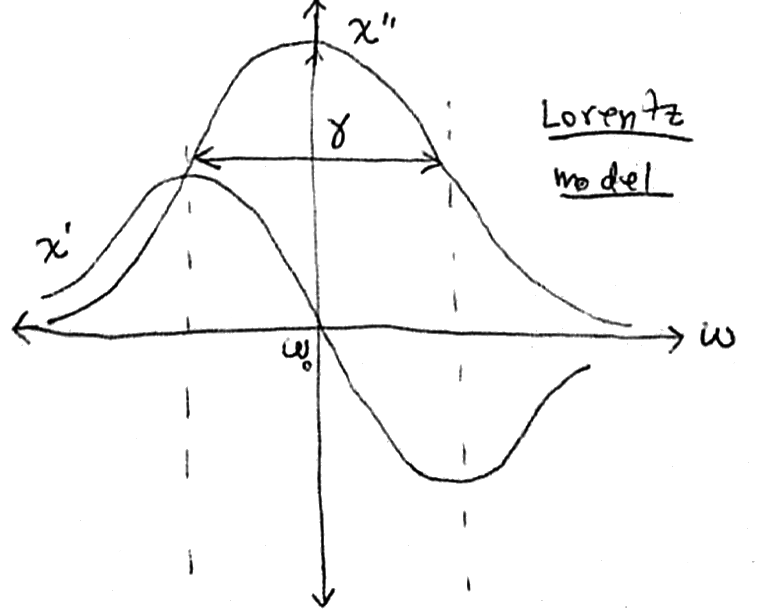
\includegraphics[width=0.6\textwidth]{./images/2-lorentz-group-vel}
	\caption{Slow and superluminal group velocities in the Lorentz model}
	\label{fig:lorentz-group-vel}
\end{figure}
